\subsubsection{Separation of Concerns}

Since the early years of software engineering, \gls{soc} has been one of the fundamental
software design principles. The concept itself was introduced by
\citeauthor{parnas_criteria_1972} with his introduction of Information Hiding
\parencite{parnas_criteria_1972}. \gls{soc} as a principle has first been mentioned by
\citeauthor{dijkstra_selected_1982}\footnote{\url{https://en.wikipedia.org/wiki/Separation_of_concerns}}
as the crucial principle to design modular software architecture
\parencite[]{dijkstra_selected_1982}. 

\gls{soc} promotes the idea that a program should be divided into distinct sections, each
addressing a separate concern or aspect of a design problem. This allows for a more
organized and maintainable source code. When implemented correctly, a change to one
concern does not affect the others. \gls{soc} should be applied at the level of individual
modules, rather that the level of an entire program.

The \gls{soc} had its effect on later versions of software design principles like SOLID.
It also influenced \gls{ns}, although it has a more strict definition of this principle.
In the book of \citeauthor{mannaert_normalized_2016} it is described as followed: 

\begin{tcolorbox}
    \begin{center}
        \textbf{Theorem I}\\
        \textit{A processing function can only contain a single task to achieve stability.}    
    \end{center}        
\end{tcolorbox}

There are various manifestations of \gls{soc} observable in the artifacts. One of which is
already mentioned in Figure \ref{fig:modulair_components}, where \gls{soc} is applied to
separate the domain logic from the application, infrastructure and presentation logic.

Another example is the separation of handlers as part of the Clean Architecture Expander.
Each of those handlers executes an isolated part of the expanding process. Consider the
\citetitle{koks_expandentitieshandlerinteractor_2023}
\parencite{koks_expandentitieshandlerinteractor_2023} for example. This Handler is solely
responsible for the generation of Data Entities. 

\begin{figure}[H]
    \centering
    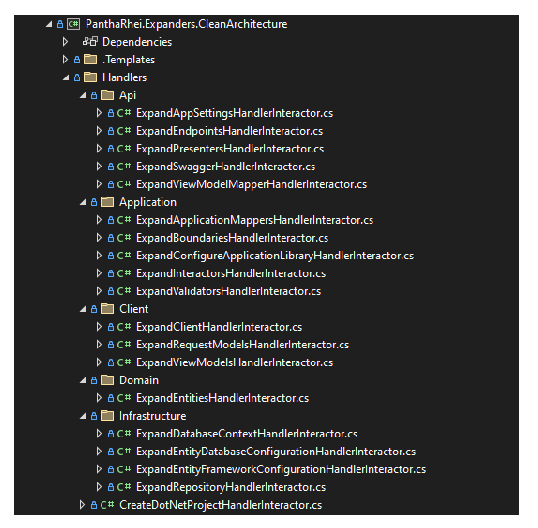
\includegraphics[width=0.8\textwidth]{Figures/expander_handlers.pdf}
    \caption[handlers]{Each of the handlers handles an isolated part of the expanding process.}
    \label{fig:handlers}
\end{figure}